\section{Бинаризация признаков}

Бинаризация признаков – это процесс преобразования исходных признаков в бинарные переменные, которые принимают значения \(0\) или \(1\). 
%Этот метод широко используется в задачах %машинного обучения, особенно в логических %методах классификации, где входные данные %должны быть представлены в виде набора %булевых предикатов.

\subsection{Бинаризация количественных признаков}

Для признака \( f: X \to D_f \), где \( D_f \) – множество возможных значений признака, бинаризация заключается в создании предикатов, проверяющих выполнение определённых условий. Эти предикаты позволяют разбить множество значений признака на подмножества, которые можно использовать в логических моделях.

В зависимости от типа признака, бинаризация осуществляется следующим образом:
\begin{itemize}
    \item \textbf{Номинальный признак} (\(f\) принимает конечное множество значений, без упорядоченности):
    \[
    \beta(x) = [f(x) = d], \quad d \in D_f;
    \]
    \[
    \beta(x) = [f(x) \in D'], \quad D' \subset D_f.
    \]
    \item \textbf{Порядковый или количественный признак} (\(f\) принимает значения, между которыми можно определить порядок):
    \[
    \beta(x) = [f(x) \leq d], \quad d \in D_f;
    \]
    \[
    \beta(x) = [d \leq f(x) \leq d'], \quad d, d' \in D_f, \, d < d'.
    \]
\end{itemize}

Для количественных признаков (\(f: X \to \mathbb{R}\)) важно выбирать такие пороговые значения \(d\), которые разделяют выборку на значимые группы. Например, 
%пороги \(d\) могут быть определены как средние значения между %соседними элементами вариационного ряда \(f(x_1), \dots, %f(x_\ell)\), упорядоченного по возрастанию:
\[
d_i = \frac{f^{(i)} + f^{(i+1)}}{2}, \quad f^{(i)} \neq f^{(i+1)}, \; i = 1, \dots, \ell - 1,
\]
где \(f^{(1)} \leq f^{(2)} \leq \dots \leq f^{(\ell)}\) – упорядоченные значения признака. (См. рис)

Такими способами можно получить много разных предикатов. Мы хотим выбрать из них самые ''лучшие'' (в каком-либо смысле). Для этого разобьем диапазон значений признака на зоны.

\begin{figure}
    \centering
    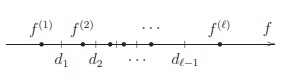
\includegraphics[scale = 1]{images/bin1.png}
    \caption{Вариационный ряд значений признака $f(x)$ и пороги $d_i$}
\end{figure}

\subsection{Разбиение диапазона значений признака на зоны}

Каждая зона определяется бинарным предикатом:
\begin{align*}
\zeta_0(x) &= [f(x) < d_1], \\
\zeta_s(x) &= [d_s \leq f(x) < d_{s+1}], \quad s = 1, \dots, r-1, \\
\zeta_r(x) &= [d_r \leq f(x)].
\end{align*}

Способы разбиения:
\begin{itemize}
    \item Жадная максимизация информативности путем слияний
    \item Разбиение на равномощные подвыборки
    \item Разбиение по равномерной сетке ''удобных'' значений (например, с минимальным числом значащих цифр)
    \item Объединение нескольких разбиений
\end{itemize}

\subsection{Жадный алгоритм слияния зон}

Алгоритм начинает с разбиения на ''мелкие'' зоны. Пороги проходят между всеми соседними парами точек, принадлежащих \emph{разным} классам, т.~к. расстановка порогов между точками одного класса приведет только к уменьшению информативности зон. Далее зоны укрупняются путём слияния \emph{троек} соседних зон. Зоны сливаются до тех пор, пока
информативность некоторой слитой зоны превышает информативность
исходных зон, либо пока не будет получено заданное количество зон $r$. Каждый раз сливается тройка, дающая наибольший выигрыш в информативности.

\begin{figure}
    \centering
    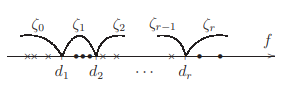
\includegraphics[scale = 1]{images/bin2.png}
    \caption{Начальное разбиение на зоны}
\end{figure}

\newpage
\textbf{Вход:}
\begin{itemize}
    \item $f(x)$ — признак;
    \item $c \in Y$ — выделенный класс;
    \item $X^\ell = \{(x_i, y_i)\}_{i=1}^\ell$ — выборка, упорядоченная по возрастанию $f(x_i)$;
    \item $r$ — желаемое количество зон;
    \item $\delta_0$ — порог слияния зон (по умолчанию $\delta_0 = 0$).
\end{itemize}

\textbf{Выход:}
\[
D = \{d_1, \dots, d_n\} \text{ — строго возрастающая последовательность порогов;}
\]

\hline

\begin{enumerate}
    \item $D := \emptyset;$
    \item \textbf{для всех} $i = 2, \dots, \ell$:
    \begin{itemize}
        \item \textbf{если} $f(x_{i-1}) \neq f(x_i)$ и $[y_{i-1} = c] \neq [y_i = c]$ \textbf{то}
        \begin{itemize}
            \item добавить новый порог $d := \frac{f(x_{i-1}) + f(x_i)}{2}$ в конец последовательности $D$;
        \end{itemize}
    \end{itemize}
    \item \textbf{повторять}
    \begin{enumerate}
        \item \textbf{для всех} $d_i \in D, i = 1, \dots, |D| - 1$:
        \begin{itemize}
            \item вычислить выигрыш от слияния тройки соседних зон $\zeta_{i-1}, \zeta_i, \zeta_{i+1}$:
            \[
            \delta_i := I_c(\zeta_{i-1} \cup \zeta_i \cup \zeta_{i+1}) - \max\{I_c(\zeta_{i-1}), I_c(\zeta_i), I_c(\zeta_{i+1})\};
            \]
        \end{itemize}
        \item найти тройку зон, для которой слияние наиболее выгодно:
        \[
        i := \arg \max \delta_i;
        \]
        \item \textbf{если} $\delta_i > \delta_0$ \textbf{то}
        \begin{itemize}
            \item слить зоны $\zeta_{i-1}, \zeta_i, \zeta_{i+1}$, удалить пороги $d_i$ и $d_{i+1}$ из последовательности $D$;
        \end{itemize}
    \end{enumerate}
    \item \textbf{пока} $|D| > r + 1$.
\end{enumerate}

\subsection{Задачи}

\textbf{Задача 1}
Предположим, вы владелец интернет-магазина, и у вас есть данные о стоимости товаров и их популярности (популярен — \( 1 \), непопулярен — \( 0 \)). 
Для анализа спроса вы хотите разбить товары на ценовые зоны, чтобы лучше понять поведение покупателей.

Данные представлены в таблице:

\[
\begin{array}{|c|c|c|}
\hline
\text{№ товара} & \text{Цена товара (\$)} & \text{Популярность } y \\
\hline
1 & 10 & 1 \\
2 & 12 & 1 \\
3 & 15 & 0 \\
4 & 17 & 1 \\
5 & 20 & 0 \\
6 & 23 & 0 \\
7 & 25 & 1 \\
\hline
\end{array}
\]

Как алгоритм слияния зон первично разобьёт выборку на ценовые зоны?

\textbf{Решение}
Рассчитаем пороги:

\[
\begin{aligned}
&d_1 = \frac{12 + 15}{2} = 13.5, \\
&d_2 = \frac{15 + 17}{2} = 16.0, \\
&d_3 = \frac{17 + 20}{2} = 18.5, \\
&d_4 = \frac{23 + 25}{2} = 24.0
\end{aligned}
\]

На основе рассчитанных порогов получаем зоны:

\[
\begin{aligned}
&\zeta_0(x) = [\text{Цена} < 13.5], \\
&\zeta_1(x) = [13.5 \leq \text{Цена} < 16.0], \\
&\zeta_2(x) = [16.0 \leq \text{Цена} < 18.5], \\
&\zeta_4(x) = [29.0 \leq \text{Цена} < 24.0], \\
&\zeta_5(x) = [\text{Цена} \geq 24.0].
\end{aligned}
\]

\textbf{Задача 2}
Будут ли разбиения диапазона меняться в зависимости от класса, относительно которого они производятся? Как изменить алгоритм для получения ''универсального'' разбиения, учитывающего сразу все классы? 

\textbf{Решение}
Да, будут, т.~к. информативность зависит от класса. Нужно заменить критерий информативности многоклассовым критерием.

\textbf{Задача 3}
Какую сложность имеет алгоритм слияния зон? Как можно его ускорить?

\textbf{Решение}
Этот алгоритм имеет трудоёмкость $O(l^2)$. Его можно заметно ускорить, если на каждой итерации сливать не одну тройку зон, а $\tau l$ троек с достаточно большим выигрышем $\delta I_i$, при условии, что они не перекрываются. В этом случае трудоёмкость составляет $O(l / \sqrt{\tau})$.
